\documentclass[tikz,border=10pt]{standalone}
\begin{document}
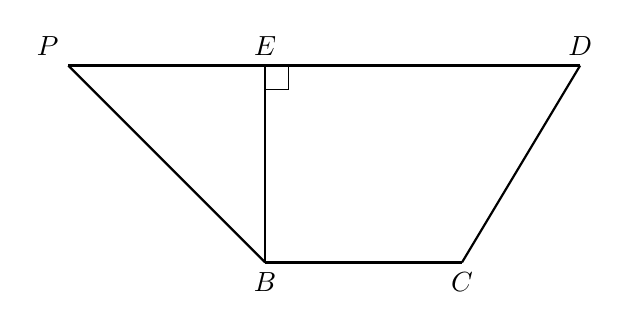
\begin{tikzpicture}
\coordinate (P) at (0,3);
\coordinate (E) at (2.5,3);
\coordinate (D) at (6.5,3);
\coordinate (B) at (2.5,0.5);
\coordinate (C) at (5,0.5);
\draw[thick] (P) -- (D);
\draw[thick] (P) -- (B);
\draw[thick] (B) -- (E);
\draw[thick] (B) -- (C);
\draw[thick] (C) -- (D);
\draw (2.5,2.7) -- (2.8,2.7) -- (2.8,3);
\node[above left] at (P) {$P$};
\node[above] at (E) {$E$};
\node[above] at (D) {$D$};
\node[below] at (B) {$B$};
\node[below] at (C) {$C$};
\end{tikzpicture}
\end{document}
